
\documentclass[12pt]{article}
\setlength\parindent{0pt}
\usepackage{fullpage}
\usepackage{xcolor}
\usepackage{amsmath}
\usepackage[margin=1in]{geometry}
\usepackage{graphicx}
\setlength{\parskip}{4mm}
\def\LL{\left\langle}   % left angle bracket
\def\RR{\right\rangle}  % right angle bracket
\def\LP{\left(}         % left parenthesis
\def\RP{\right)}        % right parenthesis
\def\LB{\left\{}        % left curly bracket
\def\RB{\right\}}       % right curly bracket
\definecolor{Red}           {rgb}{1,0.4,0.4}
\def\PAR#1#2{ {{\partial #1}\over{\partial #2}} }
\def\PARTWO#1#2{ {{\partial^2 #1}\over{\partial #2}^2} }
\def\PARTWOMIX#1#2#3{ {{\partial^2 #1}\over{\partial #2 \partial #3}} }
\newcommand{\BE}{\begin{displaymath}}
\newcommand{\EE}{\end{displaymath}}
\newcommand{\BNE}{\begin{equation}}
\newcommand{\ENE}{\end{equation}}
\newcommand{\BEA}{\begin{eqnarray}}
\newcommand{\EEA}{\nonumber\end{eqnarray}}
\newcommand{\EL}{\nonumber\\}
\newcommand{\la}[1]{\label{#1}}
\newcommand{\ie}{{\em i.e.\ }}
\newcommand{\eg}{{\em e.\,g.\ }}
\newcommand{\cf}{cf.\ }
\newcommand{\etc}{etc.\ }
\newcommand{\Tr}{{\rm tr}}
\newcommand{\etal}{{\it et al.}}
\newcommand{\OL}[1]{\overline{#1}\ } % overline
\newcommand{\OLL}[1]{\overline{\overline{#1}}\ } % double overline
\newcommand{\OON}{\frac{1}{N}} % "one over N"
\newcommand{\OOX}[1]{\frac{1}{#1}} % "one over X"

\pagenumbering{gobble}

\begin{document}
\Large
\centerline{\sc{Recitation Exercises}}
\normalsize
\centerline{\sc{Friday, 25 March}}
%
%
%{A rock climber of mass 70 kg is climbing a cliff face when she slips and falls. She is two meters above her last anchor, so she will undergo free fall for 4 meters before the rope begins to arrest her fall. If the stiffness in her rope is 1400 N/m, then:}
%  \begin{enumerate}
%    \item{How far will she fall in total?}
%\vspace{2in}
%
%    \item{What is the maximum force that her rope will exert on her as it arrests her fall?}
%\vspace{1.5in}
%
%    \item When would it be desirable for a rock climber to use a rope with a large spring constant? What about a smaller spring constant? You'll need to think about 
%          the engineering reasons for climbers to use ropes at all: the goal is to minimize the forces involved in arresting a climber's fall.
%   \end{enumerate}
%
%\newpage
%%
%% \item{A laptop battery says it has a capacity of 51 ``watt-hours''.}
%%   \begin{enumerate}
%%     \item{What are the dimensions of this odd unit ``watt-hour'', and what does it measure? What is 51 watt-hours in more familiar units?}
%%
%%\vspace{2.5in}
%%
%%     \item{If this battery were used to power an electric motor, how high could it lift the battery? Assume the battery has a mass of 300 grams.}
%%\vspace{2.5in}
%%   \end{enumerate}
%%
%%\newpage

\begin{center}
	\small \it If you didn't get to this problem Wednesday, do it today.
\end{center}

 An object rests at bottom of an incline that is elevated at an angle $\theta$ above the horizontal. Suppose that there is no friction at first. A person slides this object up the incline; it travels a distance $D$ up the incline before it slides back down.

\begin{enumerate}

\item What forces act on the object? Determine whether each one does positive work, negative work, or zero work on the way up and on the way down.

{\color{Red}Gravity does negative work on the way up and positive work on the way down. The normal force does no work since it is perpendicular to the motion.}


\item	Suppose at first there is no friction. What initial velocity does the person have to slide it with for it to travel a distance $D$ before it begins to slide back down? 

{\color{Red}
	
	Work-energy theorem:
	
	$$\frac{1}{2}mv_0^2 + W_{all} = \frac{1}{2}mv_f^2$$
	
	But $v_f=0$ and the only force doing work is gravity, so
	
	$$\frac{1}{2}mv_0^2 - mgd\sin \theta = 0 \rightarrow v_0 = \sqrt{2gd\sin \theta}$$
}


\item	When it reaches the base of the incline again, how will its velocity compare to the initial velocity that it had on the way up? {\it (You should be able to answer this without doing any mathematics.)}

{\color{Red}It'll be the same since gravity is conservative.}

\item	Now, suppose that there is friction -- a coefficient of friction $\mu_k$ between the ramp and the object. 
What initial velocity would the person have to slide it with {\it now} for it to travel a distance $D$ before it comes back down?

{\color{Red} Now we add the work done by friction. The force of friction is $\mu mg \cos \theta$ and the thing slides a distance $d$; there is no trigonometric factor here in the dot product since the force and displacement are exactly opposite.
	
	
	$$\frac{1}{2}mv_0^2 - mgd\sin \theta - \mu mgd \cos \theta = 0$$
	
	Solve for $v_0$: $$v_0 = \sqrt{2gd\sin \theta + 2\mu gd \cos \theta}.$$
	
}


\item How fast will it be moving {\it now} when it reaches the bottom of the ramp? 

{\color{Red} The hard way to do this is to write down the work-energy theorem from start to finish -- noting here that the work done by gravity is zero (since it does negative work on the way up and positive work on the way down), but that kinetic friction does negative work both ways (so $W_f = 2 \mu mgd \cos \theta$). The easier way to do it is to observe that it starts at rest at the top of the ramp, and just write the work-energy theorem
	for the way down:
	
	$$0 + mgd \sin \theta - \mu mgd \cos \theta = \frac{1}{2}mv_f^2 \rightarrow v_f = \sqrt{2gd \sin \theta - 2\mu gd \cos \theta}$$
}

\item If an object travels through some path but comes back to where it starts, like in this case, a force that always does zero work is a {\it conservative force}. A force that does do work when an object travels along a closed path is a {\it nonconservative force}.

Three forces appear in this problem: a normal force, gravity, and friction. Is each of these a conservative force? Why or why not?

{\color{Red}Gravity is conservative; friction is nonconservative; the normal force doesn't do any work at all so it's silly to talk about either one.}

\end{enumerate}
\newpage

 
 A child is swinging on a tire swing hanging from a tree. The swing has a length $L$, and the
 	tire plus the child have a mass $m$.
 	
 	The child's older sibling pulls the swing back to an angle $\theta$ and releases it from position A.
 	
 	However, a strong wind is blowing from left to right, exerting a constant horizontal force $F_w$ on the swing to the right. This means that it will swing to a larger angle $\phi$ on the right (at position~C) than it started on the left.




 	\begin{center}
 		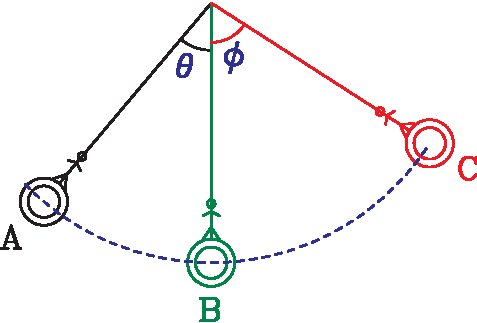
\includegraphics[width=0.6\textwidth]{swing-crop.pdf}
 	\end{center}

 
   \begin{enumerate}
 	\item Write an equation for the work-energy theorem as the swing moves from A to B. Label in words what each term represents, using language as ``kinetic energy at point A'', ``potential energy at point B'', or ``work done by wind in moving from A to B''.
 	
{\color{Red} This looks gross but it's not. The key is to realize that the work done by gravity depends only on the vertical motion (change in y) and the work done by the wind depends only on the horizontal motion (change in x).
	Also note that the distance moved down is $L - L \cos \theta$.

So the work-energy theorem is

$$0 + (L - L \cos \theta) mg + L \sin \theta F_w = \frac{1}{2}mv_B^2.$$

}
 	\item Find the speed of the swing at position B in terms of $F_w$, $m$, $L$, $\theta$, and $g$.
 	
 	{\color{Red} Do maffs:
 		
 		$$0 + (L - L \cos \theta) mg + L \sin \theta F_w = \frac{1}{2}mv_B^2$$
 		
 		$$v_B = \sqrt {2g(L - L \cos \theta) + \frac{2}{m} L \sin \theta F_w}$$
 		
 	}
 	
 	
 	\item Write down an equation that you could solve for the angle $\phi$ in terms of $F_w$, $m$, $L$, $\theta$, and $g$. (You do not need to actually solve it.) As before, label each term that appears in your expression for the work-energy theorem.
 	
 	{\color{Red} Here you could write down the work-energy theorem from B to C and use the $v_B$ above, but it is simpler to just do it from A to C. Note that the distance moved down on the left is $L - L \cos \theta$ and the distance moved up on the right is $L - L \sin \theta$, so we are moving upward in net $L - L \cos \theta - (L - L \cos \phi) = L \cos \phi - L \sin \theta$. This means that the work done by gravity is $-mg \Delta y = mg(L \cos \theta - L \cos \phi)$.
 		
 		So now we write down the work-energy theorem from A to C:
 		
 		$$
 		0 + F_w(L \sin \theta + L \sin \phi) + mg(L \cos \theta - L \cos \phi) = 0
 		$$
 		
 		and that's all they need to do!
 	}
 		
 	
 	
 	\item When the tire swings back to the left, will it stop at position $A$, will it move further to the left, or will it not reach position $A$ at all? In deciding this, think about the work done by each force as the tire swings from A to C and then back to A. Call your coach or TA over to discuss with your group.
 	
 	
 	{\color{Red} Both forces are conservative: the wind does positive work going to the right and negative work on the way back.}
 	
 \end{enumerate}
 


 \end{document}
